\documentclass{article}
\usepackage{listings}
\usepackage{color}
\usepackage{graphicx}
\usepackage{booktabs}
\usepackage{fancyhdr}
\usepackage{enumitem}
\usepackage[T1]{fontenc}
\usepackage[english]{babel}
\pagestyle{fancy}
\fancyhf{}
\rhead{
\includegraphics[width=5cm, height=0.9cm]{Images/TS_Logo}}
\lhead{GITLAB STEPS AND COMMANDS}
\lfoot{COPYRIGHT ©TALENTSPRINT, 2021. ALL RIGHTS RESERVED.}
\rfoot{\thepage}

\begin{document}
\begin{description}[style=nextline]
\item[Gitlab Steps and Commands]

The following is a list of steps and common commands used to perform operations in gitlab. Steps 1-4 are used only the first time that the gitlab set up is performed with your credentials. Step 5 is used only when a new repository is cloned from gitlab to the local system. Step 7 consists of the most commonly used commands for gitlab operations.

\item[1. Create a Giltab account and save the credentials.]


\item[2. Install Git on your system: https://git-scm.com/downloads]

\item[3. After installing you can use either Git Bash or Command Prompt to execute Git commands.]

\item[4. Introduce yourself to Git with your name and public email address before doing any operation.] 
The easiest way to do so is to use below commands with your credentials:

{\color{magenta}git config --global user.name "{\color{blue}Your Name Comes Here}"}

{\color{magenta}git config --global user.email} {\color{blue}you@yourdomain.example.com}


\item[5. To clone a repository in your system:]

\item Obtain the repository path from the gitlab repository by copying URL from under the ‘Clone’ tab of the repository as shown below:

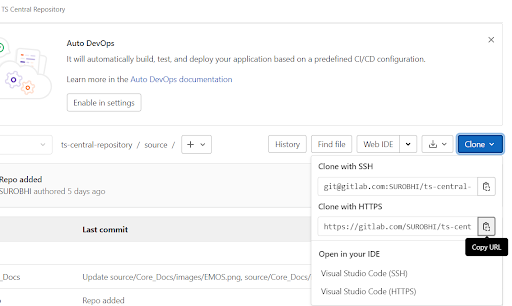
\includegraphics[width=10cm, height=6cm]{Images/GitCloneRepo_snip}

\item Open Git Bash or Command Prompt
\item Select the folder/location where you want to clone it
\item Then run below command

{\color{magenta}git clone} {\color{blue}repository path}


\item[6. To change current branch:]
A repository may have multiple branches. To check which branch we are at currently, run the following:

{\color{magenta}git status}

\item[7. To push changes in a file from your local system to the repository:]

\item Synchronize your local system with repository by using the command:

{\color{magenta}git pull}

\item Open the file in your local system and make changes to it
\item Then run these commands

{\color{magenta}        git add {\color{blue}file name with extension}

	git commit -m “{\color{blue}write commit message here}”

	git push}

In above lines,

\emph{git add}: will stage the changes to be made

\emph{git commit}: will commit the changes

\emph{git push}: will push the changes to the repository

\item[8. To change the current branch to some other branch, use below command]

{\color{magenta}git checkout {\color{blue}other branch name}}


\item[References:]

https://docs.gitlab.com/ee/gitlab-basics/start-using-git.html

https://rogerdudler.github.io/git-guide/

https://docs.gitlab.com/ee/gitlab-basics/command-line-commands.html

https://git-scm.com/docs/gittutorial 

\end{description}
\end{document}


















